% This is part of Mes notes de mathématique
% Copyright (c) 2011-2014
%   Laurent Claessens
% See the file fdl-1.3.txt for copying conditions.

%+++++++++++++++++++++++++++++++++++++++++++++++++++++++++++++++++++++++++++++++++++++++++++++++++++++++++++++++++++++++++++
\section{Généralités}
%+++++++++++++++++++++++++++++++++++++++++++++++++++++++++++++++++++++++++++++++++++++++++++++++++++++++++++++++++++++++++++

\begin{definition}  \label{DefTMNooKXHUd}
    Un \defe{corps}{corps} est un anneau non nul dans lequel tout élément non nul est inversible.
\end{definition}

\begin{remark}
    Nous trouvons parfois le terme \defe{anneau à division}{anneau!à division}. Cela provient du fait que dans beaucoup de cas on considère uniquement des corps commutatifs; donc on voudrait une façon de parler d'un anneau dont tous les éléments non nuls sont inversibles. Dans ce cadre on dit :
    \begin{itemize}
        \item Un anneau à division est un anneau dont tous les éléments non nuls sont inversibles,
        \item Un corps est un anneau à division commutatif.
    \end{itemize}
    Pour prendre un exemple de cette différence, le théorème de Wedderburn \ref{ThoMncIWA} est énoncé ici sous les termes «Tout corps fini est commutatif». Sous-entendu : la commutativité ne fait pas partie de la définition d'un corps. Par contre dans \cite{KXjFWKA} il est énoncé sous les termes «Tout anneau à division fini est un corps». Chez lui, un corps est toujours commutatif et un anneau à division est ce que nous appelons ici un corps.
    
    Dans tous les cas, un corps dans lequel l'élément nul est inversible est appelé un mensonge, comme le prouve le lemme suivant.
\end{remark}

\begin{lemma}       \label{LemAnnCorpsnonInterdivzer}
    En tant que anneau, un corps n'a pas de diviseurs zéro.
\end{lemma}

\begin{proof}
    En effet si \( a\) est un diviseur de zéro, alors \( ax=0\) pour un certain \( x\neq 0\). Si \( a\) était inversible, nous aurions \( x=a^{-1}ax=0\), ce qui est impossible.
\end{proof}

\begin{definition}[Algèbre\cite{ZSyHmiy}]   \label{DefAEbnJqI}
    Si \( \eK\) est un corps commutatif\footnote{Définition \ref{DefTMNooKXHUd}}, une \( \eK\)-\defe{algèbre}{algèbre} \( A\) est un espace vectoriel muni d'une opération bilinéaire \( \times\colon A\times A\to A\), c'est à dire telle que pour tout \( x,y,z\in A\) et pour tout \( \alpha,\beta\in\eK\),
    \begin{enumerate}
        \item
            \( (x+y)\times z=x\times z+y\times z\)
        \item
            \( x\times (y+z)=x\times y+x\times z\)
        \item
            \( (\alpha x)\times (\beta y)=(\alpha\beta)(x\times y)\).
    \end{enumerate}
    Si \( A\) et \( B\) sont deux \( \eK\)-algèbres, une application \( f\colon A\to B\) est un \defe{morphisme}{morphisme!d'algèbres} entre \( A\) et \( B\) si pour tout \( x,y\in A\) et pour tout \( \alpha\in \eK\),
    \begin{enumerate}
        \item
            \( f(xy)=f(x)f(y)\)
        \item
            \( f(x+\alpha y)=f(x)+\alpha f(y)\)
    \end{enumerate}
    où nous avons noté \( xy\) pour \( x\times y\).
\end{definition}


Par le lemme \ref{LemCaractIntergernbrcartpre}, un anneau sans diviseur de zéro est de caractéristique zéro ou première. Le fait d'être intègre pour un anneau n'assure cependant pas le fait d'être un corps. Nous avons cependant ce résultat pour les anneaux finis.

\begin{proposition}     \label{PropanfinintimpCorp}
    Un anneau fini intègre est un corps.
\end{proposition}

\begin{proof}
    Soit \( A\) un tel anneau. Soit \( a\neq 0\). Les applications 
    \begin{subequations}
        \begin{align}
            l_a\colon x\to ax\\
            r_a\colon x\to xa
        \end{align}
    \end{subequations}
    sont injectives. En tant que applications injectives entre ensembles finis, elles sont surjectives. Il existe donc \( b\) et \( c\) tels que \( 1=ba=ac\). Il se fait que \( b\) et \( c\) sont égaux parce que
    \begin{equation}
        b=b(ac)=(ba)c=c.
    \end{equation}
    Par conséquent \( b\) est un inverse de \( a\).
\end{proof}

\begin{proposition}     \label{PropzhFgNJ}
    Soit \( n\in\eN^*\). Les conditions suivantes sont équivalentes :
    \begin{enumerate}
        \item
            \( n\) est premier.
        \item
            \( \eZ/n\eZ\) est un anneau intègre.
        \item
            \( \eZ/n\eZ\) est un corps.
    \end{enumerate}
\end{proposition}

\begin{proof}
    L'équivalence entre les deux premiers points est le contenu du corollaire \ref{CorZnInternprem}. Le fait que \( \eZ/n\eZ\) soit un corps lorsque \( \eZ/n\eZ\) est intègre est la proposition \ref{PropanfinintimpCorp}. Le fait que \( \eZ/n\eZ\) soit intègre lorsque \( \eZ/n\eZ\) est un corps est une propriété générale des corps : ce sont en particulier des anneaux intègres (lemme \ref{LemAnnCorpsnonInterdivzer}).
\end{proof}

\begin{proposition}     \label{AnnCorpsIdeal}
    Si \( A\) est un anneau, nous avons les équivalences
    \begin{enumerate}
        \item
            \( A\) est un corps.
        \item
            \( A\) est non nul et ses seuls idéaux à gauche sont \( \{ 0 \}\) et \( A\).
        \item
            \( A\) est non nul et ses seuls idéaux à droite sont \( \{ 0 \}\) et \( A\).
    \end{enumerate}
\end{proposition}

\begin{proposition}
    Soit \( A\), un anneau commutatif non nul et \( I\), un idéal dans \( A\). L'ensemble \( I\) est un idéal maximum de \( A\) si et seulement si \( A/I\) est un corps.
\end{proposition}

\begin{proof}
    Par la proposition \ref{AnnCorpsIdeal}, le fait pour \( A/I\) d'être un corps signifie qu'il n'a pas d'idéaux non triviaux. Si \( \phi\) est la projection canonique \( A\mapsto A/I\), nous savons que les idéaux de \( A/I\) sont les \( \phi(J)\) où \( J\) est un idéal de \( A\) contenant \( I\) (proposition \ref{PropIJJIdsousphi}). Si \( I\) est un idéal maximum de \( A\), un tel \( J\) n'existe pas. Inversement si \( A/I\) n'a pas d'autres idéaux que \( A/I\) et \( \phi(0)\), c'est que \( I\) est un idéal maximum.
\end{proof}

%---------------------------------------------------------------------------------------------------------------------------
\subsection{Corps des fractions}
%---------------------------------------------------------------------------------------------------------------------------

\begin{theorem}     \label{ThogbhWgo}
    Soit \( \eA\) un anneau commutatif intègre. Il existe un corps commutatif \( \eK\) et un morphisme injectif (d'anneaux) \( \epsilon\colon \eA\to \eK\) tels que pour tout \( \lambda\in\eK\), il existe \( (a,b)\in \eA\times \eA^*\) tels que
    \begin{equation}
        \lambda=\epsilon(a)\big( \epsilon(b) \big)^{-1}
    \end{equation}

    De plus si \( (\eK',\epsilon')\) est un autre couple qui vérifie la propriété, les corps \( \eK\) et \( \eK'\) sont isomorphes.
\end{theorem}
Le corps \( \eK\) associé à l'anneau \( \eA\) est le \defe{corps des fractions}{corps!des fractions}\index{fractions (corps)} de \( \eA\), et sera noté \( \Frac(\eA)\).\nomenclature[A]{\( \Frac(\eA)\)}{Le corps des fractions de l'anneau \( \eA\)}

Notons que l'application \( \eA\times \eA^*\to \eK\) donnée par \( (a,b)\mapsto \epsilon(a)\big( \epsilon(b) \big)^{-1}\) envoie \( (xa,xb)\) sur le même que \( (a,b)\).

L'ensemble \( \eQ\)\nomenclature[A]{\( \eQ\)}{corps des fractions sur \( \eZ\)} est le corps des fractions de \( \eZ\).

%---------------------------------------------------------------------------------------------------------------------------
\subsection{Corps premier}
%---------------------------------------------------------------------------------------------------------------------------
\label{subseccorpspremhBlYIv}

\begin{definition}
    Un corps est \defe{premier}{corps!premier}\index{premier!corps} si il est son seul sous corps. Le \defe{sous corps premier}{premier!sous corps} d'un corps est l'intersection de tous ses sous corps.
\end{definition}

\begin{lemma}
    Un corps premier est commutatif
\end{lemma}

\begin{proof}
    Le centre d'un corps est certainement un sous corps. Par conséquent un corps premier doit être contenu dans son propre centre, c'est à dire être commutatif.
\end{proof}

Soit \( p\) un nombre premier. Nous notons \( \eF_p=\eZ_p=\eZ/p\eZ\)\nomenclature[A]{\( \eF_p\)}{lorsque \( p\) est premier}. Nous verrons plus loin (section \ref{SecCorpsFinizkAcbS}) comment nous pouvons définir \( \eF_{p^n}\) lorsque \( p\) est premier.

Nous avons par exemple 
\begin{equation}
    \eF_2=\eZ/2\eZ=\{ 0,1 \}
\end{equation}
avec la loi \( 2=0\).

Notons que \( \eF_p\) est un corps possédant \( p\) éléments. L'ensemble \( \eF_p^*\) est un groupe d'ordre \( p-1\).

\begin{lemma}
    Les corps \( \eQ\) et \( \eF_p\) (avec \( p\) premier) sont premiers.
\end{lemma}

\begin{proof}
    Tout sous corps de \( \eQ\) doit contenir \( 1\), et par conséquent \( \eZ\). Devant également contenir tous les inverses, il contient \( \eQ\).

    Tout sous corps de \(\eF_p \) doit contenir \( 1\) et donc \( \eF_p\) en entier. Par ailleurs nous savons de la proposition \ref{PropzhFgNJ} que \( \eF_p\) est un corps lorsque \( p\) est premier.
\end{proof}

\begin{proposition}
    Soit \( \eK\) un corps de caractéristique \( p\) et \( \eP\) son sous corps premier. Si \( p=0\) alors \( \eP=\eQ\). Si \( p>0\), alors \( \eP=\eF_p\).
\end{proposition}

\begin{proof}
    Notons d'abord que la caractéristique d'un corps est toujours un nombre premier parce qu'un corps est en particulier un anneau intègre (proposition \ref{LemCaractIntergernbrcartpre}).

    Étant donné que \( 1\) est dans tout sous corps, nous devons avoir \( \eZ 1\subseteq \eP\). Si \( p=0\), alors \( \eZ 1\simeq \eZ\), et nous avons
    \begin{equation}
        \eZ 1_{\eA}\subset \eP\subset \eK.
    \end{equation}
    Pour chaque \( (n,m)\in \eZ 1_{\eA}\times (\eZ 1_{\eA})^*\) l'élément \( nm^{-1}\in \eK\) est dans \( \eP\) parce que \( \eP\) est un corps. Nous en déduisons que le corps des fractions de \( \eZ\) est contenu dans \( \eP\) par conséquent \( \eP=\eQ\) (théorème \ref{ThogbhWgo}). 

    Si par contre la caractéristique de \( \eK\) est \( p\neq 0\), nous avons \( \eZ 1_{\eA}\simeq\eZ/p\eZ=\eF_p\) par le lemme \ref{LemHmDaYH}. L'ensemble \( \eF_p\) étant un corps, c'est le corps premier de \( \eK\).
\end{proof}

\begin{proposition}     \label{PropqPPrgJ}
    Soit \( \eK\) un corps et \( \eP\) sont sous corps premier. Si \( \sigma\in\Aut(\eK)\) alors \( \sigma|_{\eP}=\id\), c'est à dire que
    \begin{equation}
        \sigma(x)=x
    \end{equation}
    pour tout \( x\in \eP\).
\end{proposition}

\begin{theorem}[Théorème de Gauss]  \label{ThoLLgIsig}
    Soient \( P,Q,R\in \eK[X]\) tels que \( P\) soit premier avec \( Q\) et divise \( QR\). Alors \( P\) divise \( R\).
\end{theorem}
\index{théorème!Gauss!polynômes}

\begin{proof}
    Étant donné que \( P\) est premier avec \( Q\), le théorème de Bézout\footnote{théorème \ref{ThoBezoutOuGmLB}.} nous donne \( U,V\in \eK[X]\) tels que \( PU+QV=1\). De plus il existe un polynôme \( S\) tel que \( PS=QR\). En multipliant l'identité de Bézout par \( R\), nous obtenons
    \begin{equation}
        R=PUR+QVR=PUR+VPS=P(UR+VS),
    \end{equation}
    ce qui signifie que \( P\) divise \( R\).
\end{proof}

Le lemme suivant est une généralisation du lemme de Gauss dans \( \eZ\) (lemme \ref{LemSdnZNX}).
\begin{lemma}[Lemme de Gauss\cite{fJhCTE}]       \label{LemEfdkZw}   \index{lemme!Gauss!polynômes}\index{Gauss!lemme!polynômes}
    Soient les polynômes unitaires \( P,Q\in \eQ[X]\). Si \( PQ\in\eZ[X]\), alors \( P\) et \( Q\) sont tous deux dans \( \eZ[X]\).
\end{lemma}

\begin{proof}
    Soit \( a>0\) le plus petit entier tel que \( aP\in\eZ[X]\) (c'est le PPCM des dénominateurs) et de la même façon \( b>0\) le plus petit entier tel que \( bQ\in \eZ[X]\). On pose \( P_1=aP\) et \( Q_1=bQ\).

    Si \( ab=1\), alors \( a=b=1\) et nous avons tout de suite \( P,Q\in \eZ[X]\). Nous supposons donc \( ab>1\) et nous considérons \( p\), un diviseur premier de \( ab\). Ensuite nous considérons la projection
    \begin{equation}
        \pi_p\colon \eZ[X]\to (\eZ/p\eZ)[X].
    \end{equation}
    Par définition \( abPQ=P_1Q_1\in \eZ[X]\); en prenant la projection,
    \begin{equation}
        \pi_p(P_1)\pi_p(Q_1)=\pi_p(P_1Q_1)=\pi_P(ab)\pi_p(PQ)=0
    \end{equation}
    parce que \( \pi_p(ab)=0\). Étant donné que \( (\eZ/p\eZ)[X]\) est intègre (exemple \ref{ExybCZyl}), nous avons soit \( \pi_p(P_1)=0\) soit \( \pi_p(Q_1)=0\). Supposons pour fixer les idées que \( \pi_p(P_1)=0\). Alors \( P_1=pP_2\) pour un certain \( P_2\in \eZ[X]\). Par ailleurs \( P\) est unitaire et \( P_1=aP\), donc le coefficient de plus haut degré de \( P_1\) est \( a\), et nous concluons que \( p\) divise \( a\).
    
    Mettons \( a=pa'\). Dans ce cas, \( pa'P=P_1=pP_2\), et donc \( a'P=P_2\in \eZ[X]\). Cela contredit la minimalité de \( a\).
\end{proof}

%---------------------------------------------------------------------------------------------------------------------------
\subsection{Petit théorème de Fermat}
%---------------------------------------------------------------------------------------------------------------------------

\begin{theorem}[Petit théorème de Fermat]       \label{ThoOPQOiO}   \index{théorème!petit de Fermat}\index{petit théorème de Fermat}
    Soit \( p\) un nombre premier. Si \( x\in \eF_p\) alors \( x^p=x\). Si \( x\in(\eF_p)^*\), alors \( x^{p-1}=1\).

    En particulier si \( x\in \eF_p^*\) alors \( x^{-1}=x^{p-2}\).
\end{theorem}

\begin{proof}
    Étant donné que \( \eF_p\) est un corps commutatif et que \( p\) est premier, la proposition \ref{Propqrrdem} nous indique que \( \sigma(x)=x^p\) est un automorphisme. La proposition \ref{PropqPPrgJ} nous indique alors que
    \begin{equation}
        a^p=a.
    \end{equation}
    Si \( a\) est inversible alors \( a^{p-1}=a^pa^{-1}=1\).
\end{proof}

\begin{remark}      \label{RemCoSnxh}
    Une autre façon d'énoncer le petit théorème de Fermat \ref{ThoOPQOiO} est que si \( p\) est premier et si \( a\) est premier avec \( a\), alors \( a^{p-1}\in[1]_p\). Le nombre \( a\) n'est pas premier avec \( p\) uniquement lorsque \( a\) est multiple de \( p\). Dans ce cas c'est \( a=0\) dans \( \eF_p\) et donc \( a^{p-1=0}\).
\end{remark}

\begin{example}
    Soit \( \eK=\eF_{29}^*\). Le nombre \( 29\) étant premier, \( \eK\) est un corps premier. C'est le corps des entier modulo \( 29\). Nous avons donc
    \begin{equation}
            -142=-113=-84=-55=-26=3=32=61=90=119.
    \end{equation}
    Le petit théorème de Fermat nous permet aussi de calculer des exposants et des inverses. Nous avons
    \begin{equation}
        x^{-a}=(x^a)^{27}=x^{27a}.
    \end{equation}
    Le nombre \( 27 a\) peut être grand par rapport à \( 29\). Étant donné que \( 1=x^{28}\) nous avons
    \begin{equation}
        x^{-a}=x^{27 a\mod 28}.
    \end{equation}
    Dans les exposants nous calculons modulo \( 28\).
\end{example}

%---------------------------------------------------------------------------------------------------------------------------
\subsection{Résultats chinois}
%---------------------------------------------------------------------------------------------------------------------------

Nous allons maintenant parler du système d'équations
\begin{subequations}
    \begin{numcases}{}
        x=a_1\mod p\\
        x=a_2\mod q
    \end{numcases}
\end{subequations}
avec \( a_1\), \( a_2\) donnés dans \( \eZ\) et \( p,q\) des entiers premiers entre eux. Le lemme chinois nous donne la liste des solutions ainsi qu'une manière de les construire. Le théorème chinois en sera une espèce de corollaire qui établira l'isomorphisme d'anneaux \( \eZ/pq\eZ\simeq \eZ/p\eZ\times \eZ/q\eZ\). Voir \href{http://www.les-mathematiques.net/b/a/d/node10.php}{les-mathematiques.net}.

\begin{lemma}[Lemme chinois \cite{CongrDuchSyl}]        \label{LemCtUeGA}
    Soient \( n_1,n_2\) deux entiers premiers entre eux. Soient \( a_1,a_2\in \eZ\). Les solutions du système
    \begin{subequations}        \label{SysVwvLKv}
        \begin{numcases}{}
            x=a_1\mod n_1\\
            x=a_2\mod n_2
        \end{numcases}
    \end{subequations}
    pour \( x\in \eZ/n_1n_2\eZ\) sont données de la façon suivante. Soient \( u_1,u_2\) deux entiers qui satisfont la relation de Bézout\footnote{voir le théorème \ref{ThoBuNjam}}
    \begin{equation}        \label{EqWcucUG}
        u_1n_1+u_2n_2=1,
    \end{equation}
    et 
    \begin{equation}        \label{EqHGchlQ}
        a=\big( a_1u_2n_2+a_2 u_1n_1 \big)\mod(n_1).
    \end{equation}
    Alors \( x=a\mod(n_1n_2)\).
\end{lemma}

\begin{proof}
    Vérifions que le \( x\) donné par \(x=a\mod(n_1n_2)\) est bien une solution. D'abord
    \begin{subequations}
        \begin{align}
            a\mod n_2&=a_1u_2n_2\mod n_1\\
            &=a_1(1-u_1n_1)\mod n_1\\
            &=a_1\mod n_1
        \end{align}
    \end{subequations}
    où nous avons utilisé l'identité de Bézout \eqref{EqWcucUG}. La vérification de \( a\mod n_2=a_2\mod n_2\) est la même.

    Soit maintenant \( x\in \eZ/n_1n_2\eZ\) une solution du système \eqref{SysVwvLKv} et \( a\) donné par la formule \eqref{EqHGchlQ}. Alors
    \begin{subequations}
        \begin{align}
            (x-a)\mod n_1&=\Big( a_1-(a_1n_2u_2+a_2u_1n_1) \Big)\mod n_1\\
            &=a_1-a_1u_2n_2\mod n_1\\
            &=0,
        \end{align}
    \end{subequations}
    donc \( (x-a)\mod n_1=0\), ce qui signifie que \( x-a\) est divisible par \( n_1\). De la même façon, \( (x-a)\mod n_2=0\) et \( x-a\) est divisible par \( n_2\). Nous savons maintenant que \( x-a\) est divisible par \( n_1\) et \( n_2\). Étant donné que \( n_1\) et \( n_2\) sont premiers entre eux, nous en déduisons que \( x-a\) est divisible par \( n_1n_2\), ou encore que \( x=a\mod n_1n_2\).
\end{proof}

\begin{theorem}[Théorème chinois]
    Soient \( p,q\) deux naturels premiers entre eux. Si \( p,q\geq 2\) alors l'application
    \begin{equation}
        \begin{aligned}
            \phi\colon \eZ/pq\eZ&\to \eZ/p\eZ\times \eZ/q\eZ \\
            [x]_{pq}&\mapsto \big( [x]_p,[x]_q \big) 
        \end{aligned}
    \end{equation}
    est un isomorphisme d'anneaux.
\end{theorem}

\begin{proof}
    Nous devons prouver que l'application \( \phi\) respecte la somme, le produit et qu'elle est bijective. En ce qui concerne la somme,
    \begin{subequations}
        \begin{align}
            \phi([q]_{pq}+[y]_{pq})&=            \phi\big( (x+y)\mod pq \big)\\
            &=\big( [x+y]_{p},[x+y]_q \big)\\
            &=\big( [x]_p+[y]_p,[x]_q+[y]_q \big)\\
            &=\big( [x]_p,[x]_q \big)+\big( [y]_p,[y]_q \big)\\
            &=\phi(x)+\phi(y).
        \end{align}
    \end{subequations}
    En ce qui concerne le produit, c'est le même jeu : nous obtenons
    \begin{equation}
        \phi\big( [xy]_{pq} \big)=\phi([x]_{pq}])\phi([y]_{pq})
    \end{equation}
    en utilisant le fait que \( [xy]_{p}=[x]_p[y]_p\).

    Montrons maintenant que \( \phi\) est surjective. Soient \( y_1,y_2\in \eZ\) et \( x\in \eZ\). Demander
    \begin{equation}
        \phi([x]_{pq})=\big( [y_1]_p,[y_2]_q \big)
    \end{equation}
    revient à demander que \( [x]_p=[y_1]_p\) et \( [x]_q=[y_2]_q\), c'est à dire que \( x\) résolve le système
    \begin{subequations}
        \begin{numcases}{}
            x=y_1\mod p\\
            x=y_2\mod q.
        \end{numcases}
    \end{subequations}
    Le lemme chinois \ref{LemCtUeGA} nous assure qu'une solution existe.

    En ce qui concerne l'injectivité, nous supposons que \( x\) et \( y\) soient deux entiers tels que
    \begin{equation}
        \phi([x]_{pq})=\phi([y]_{pq}).
    \end{equation}
    Nous en déduisons le système
    \begin{subequations}
        \begin{numcases}{}
            x\mod p=y\mod p\\
            x\mod q=y\mod q
        \end{numcases}
    \end{subequations}
    c'est à dire qu'il existe des entiers \( k\) et \( l\) tels que \( x=y+kp\) et \( x=y+lq\) ou encore tels que
    \begin{equation}
        kp+lq=0.
    \end{equation}
    Étant donné que \( p\) et \( q\) sont premiers entre eux, la seule possibilité est \( k=l=0\), c'est à dire \( x=y\).
\end{proof}

\begin{theorem}[Théorème chinois]\index{théorème!chinois}
    Soit \( A\) un anneau commutatif, \( n\geq 2\), des éléments \( x_1,\ldots,x_n\) dans \( A\) et des idéaux \( I_1,\ldots,I_n\) tels que \( I_i+I_j=A\) pour tout \( i\neq j\).

    Alors il existe un \( x\in A\) tel que \( x-x_i\in I_i\) pour tout \( 1\leq i\leq n\).
\end{theorem}

\begin{proof}
    Pour \( i\in\{ 1,\ldots,n \}\) nous notons \( J_i\) le produit \( J_i=\prod_{k\neq i}I_k\). Étant donné que chaque \( I_i\) est un idéal, nous avons \( I_k\in J_i\) lorsque \( i\neq k\).

    Soit \( i\) fixé, et considérons \( j\neq i\). Nous pouvons trouver \( a_j\in I_i\) et \( b_j\in I_j\) tel que \( a_j+b_j=1\). Nous avons alors
    \begin{equation}
        1=\prod_{j\neq i}(a_j+b_j).
    \end{equation}
    Par ailleurs \( I_i+J_i=A\) parce que \( J_i\) contient \( I_k\) avec \( k\neq i\) et \( I_i+I_k=A\). Nous pouvons donc prendre \( \alpha_i\in I_i\) et \( \beta_i\in J_i\) tels que
    \begin{equation}
        \prod_{j\neq i}(a_j+b_j)=\alpha_i+\beta_i.
    \end{equation}
    Nous considérons alors l'élément \( x=\beta_1x_1+\ldots+\beta_nx_n\) et nous avons
    \begin{subequations}
        \begin{align}
            x-x_1&=(\beta_1-1)x_1+\beta_2x_2+\ldots+\beta_nx_n\\
            &=-\alpha_1x_1+\beta_2x_2+\ldots+\beta_nx_n
        \end{align}
    \end{subequations}
    Mais \( \alpha_1\in I_1\) et tous les autres termes sont dans les \( J_i\) avec \( i\neq 1\). Par conséquent le tout est dans \( I_1\). Ici nous utilisons par exemple le fait que \( \beta_2\in J_2\subset I_1\) parce que les éléments de \( J_2\) sont des produits d'éléments dont un facteur est dans \( I_1\).
\end{proof}

\begin{remark}
    Ce théorème chinois est bien une généralisation du lemme chinois \ref{LemCtUeGA}. En effet, l'élément \( x\) dont il est question est solution du problème \( x=x_i\mod I_i\). L'hypothèse \( I_i+I_j=A\) n'est pas nouvelle non plus étant donné que si \( p\) et \( q\) sont des entiers premiers entre eux nous avons \( p\eZ+q\eZ=\eZ\) par le corollaire \ref{CorgEMtLj}.
\end{remark}

%---------------------------------------------------------------------------------------------------------------------------
\subsection{Chiffrage RSA}
%---------------------------------------------------------------------------------------------------------------------------
\label{subSecEVaFYi}
\index{groupe!fini}
\index{groupe!permutation}
\index{groupe!partie génératrice}
\index{anneau!\( \eZ/n\eZ\)}
\index{nombre!premier}

Ce passage sur RSA provient en bonne partie de la \wikipedia{fr}{Rivest_Shamir_Adleman}{la page Wikipédia}.

Alice veut envoyer un message à Bob. L'idée est que Bob va donner à Alice une clef publique qui va permettre de chiffrer le message tandis que Bob va garder pour lui une clef privée qui permet de déchiffrer.

%///////////////////////////////////////////////////////////////////////////////////////////////////////////////////////////
\subsubsection{Mise en place par Bob}
%///////////////////////////////////////////////////////////////////////////////////////////////////////////////////////////

Bob se crée une paire de clef publique, clef privée de la façon suivante.
\begin{enumerate}
    \item
        Bob choisit deux nombres premiers distincts \( p,q\).
    \item
        Il calcule \( n=pq\) .
    \item
        Par le corollaire \ref{CorlvTmsf}, l'indicatrice d'Euler \( \varphi(n)=(p-1)(q-1)\) est facile à calculer pour Bob.
    \item
        Bob choisit \( e\in \eN\) premier avec \( \varphi(n)\), puis \( d\) tel que \( ed\in[1]_{\varphi(n)}\).
\end{enumerate}
Maintenant la paire est : clef publique \( (n,e)\) et clef privée \( (n,d)\)\footnote{Le fait que \( e\) soit public et \( d\) soit privé est une convention. \( e\) comme  \emph{encryption} et \( d\) comme \emph{decryption}.}.

Bob envoie la paire \( (n,e)\) à Alice. 

\begin{remark}
    Ici nous ne supposons pas que la communication soit sure. Une tierce personne peut intercepter le message. D'ailleurs en principe les gens publient leurs clef publique sur leurs sites, voire sur des sites dédiés. Le problème de l'identification reste à résoudre \wikipedia{en}{Key_signing_party}{à l'ancienne}.
\end{remark}

%///////////////////////////////////////////////////////////////////////////////////////////////////////////////////////////
\subsubsection{Chiffrement}
%///////////////////////////////////////////////////////////////////////////////////////////////////////////////////////////

Nous chiffrons en utilisant la clef publique \( (n,e)\). D'abord Alice se débrouille pour transformer son message en un nombre plus petit que \( n\). Soit \( M\) ce message. Alice code \( M\) en
\begin{equation}
    C=M^e\mod n.
\end{equation}
Tout le truc est que nous allons voir que l'application \( x\mapsto x^e\) est une bijection de \( \eF_n\) et que l'inverse est facile à calculer par Bob et difficile pour les autres. Alice envoie \( C\) à Bob. Encore une fois, nous ne supposons pas que cette communication soit privée. Le nombre \( C\) peut être intercepté.

%///////////////////////////////////////////////////////////////////////////////////////////////////////////////////////////
\subsubsection{Déchiffrage}
%///////////////////////////////////////////////////////////////////////////////////////////////////////////////////////////

Nous allons montrer que \( M=C^d\mod n\), et donc que Bob, connaissant \( (n,d)\), peut déchiffrer. D'abord
\begin{equation}
    C^d=(M^e)^d=M^{ed},
\end{equation}
mais nous savons qu'il existe \( k\) tel que
\begin{equation}
    ed=1+k\varphi(n)=1+k(p-1)(q-1).
\end{equation}
L'étape astucieuse est de remarquer que
\begin{equation}    \label{EqreeHgn}
    M^{1+k(p-1)(q-1)}\in [M]_p\cap[M]_q.
\end{equation}
Pour montrer cela nous utilisons le petit théorème de Fermat \ref{ThoOPQOiO} et la remarque \ref{RemCoSnxh}.
\begin{itemize}
    \item Si \( M\) est premier avec \( p\), alors \( M^{p-1}\in[1]_p\).
    \item Si \( M\) n'est pas premier avec \( p\), alors \( M\) est multiple de \( p\) et on sait que \( M^{p-1}\in[0]_p=[M]_p\).
\end{itemize}
Dans les deux cas nous avons \eqref{EqreeHgn}. Le nombre \( M^{1+k\varphi(n)}-M\) est donc à la fois multiple de \( p\) et de \( q\).

Le lemme chinois \ref{LemCtUeGA} nous dit immédiatement\footnote{C'est ici qu'il est important que \( p\) ne soit pas égal à \( q\). Si \( p=q\), alors le lemme chinois ne fonctionne pas.} qu'alors
\begin{equation}
    M^{1+k\varphi(n)}-M
\end{equation}
est un multiple de \( pq=n\), c'est à dire que
\begin{equation}
    C^d=M^{ed}\in [M]_n.
\end{equation}

Si on ne croit pas au lemme chinois, on peut utiliser le lemme de Gauss. Posons
\begin{equation}
    M^{1+k\varphi(n)}-M=ap=bq.
\end{equation}
Dans ce cas \( p\) divise \( bq\), mais \( q\) est premier avec \( p\), donc le lemme de Gauss \ref{LemSdnZNX} nous enseigne\footnote{Ici aussi, si \( p=q\), ça ne marche pas.} que \( p\) divise \( b\).

%///////////////////////////////////////////////////////////////////////////////////////////////////////////////////////////
\subsubsection{Une imprudence à ne pas commettre}
%///////////////////////////////////////////////////////////////////////////////////////////////////////////////////////////

Nous avons pris deux cas selon que \( M\) soit ou non premier avec \( p\). Une question qui arrive est la suivante : est-ce que c'est une bonne idée d'envoyer un message qui ne soit pas premier avec \( p\) ?

Si nous savons que \( M\) n'est pas premier avec \( p\), alors nous avons \( M^e=l^ep^e\) et \( n=pq\) qui sont publics. Donc un calcul de PGCD permettrait de trouver \( p\).

Il faut cependant savoir que 
\begin{itemize}
    \item La probabilité que ça arrive est infime : vu que \( M\) est entre \( 0\) et \( n=pq\), les multiples de \( p\) possibles sont \( p,2p,\cdots pq\). Il y a dont une chance sur \( p\) que cela arrive. Typiquement avec des \( p\) de l'ordre de \( 10^{120}\), on peut utiliser RSA chaque milliseconde sur chaque atome de l'univers depuis le début des temps que ça ne se serait presque certainement pas encore produit.
    \item
        De toutes façons Alice ne sait pas vérifier si son message est premier avec \( p\) parce qu'elle ne connaît pas \( p\).
    \item 
        En conclusion la partie de la preuve qui montre que \( M^{1+\varphi(n)}\in [M]_p\cap[M]_q\) dans le cas \( M\) non premier avec \( p\) est, à toutes fins pratiques, inutile parce que ce cas de figure ne se présentera jamais dans toutes l'histoire de l'univers, même pas avec une civilisation intelligente autour de chaque étoile.
\end{itemize}

%///////////////////////////////////////////////////////////////////////////////////////////////////////////////////////////
\subsubsection{Problèmes calculatoires}
%///////////////////////////////////////////////////////////////////////////////////////////////////////////////////////////

Pour implémenter RSA, il faut pouvoir faire (au moins) trois choses :
\begin{enumerate}
    \item
        Trouver de grands nombres premiers.
    \item
        Trouver des couples de Bézout.
    \item
        Calculer \( M^e\) lorsque \( e\) est très grand.
\end{enumerate}
En ce qui concerne le problème de trouver des nombres premiers, c'est compliqué, mais il faut savoir qu'il y en a plein. À \( 120\) chiffres, il y a environ autant de nombres premiers que d'atomes dans \( 10^{20}\) fois l'univers connu. Cela rend impossible toute tentative de factoriser un grand nombre en essayant toutes les possibilités. Même pas en science-fiction\footnote{Cela donne une idée des connaissances en math des klingons, dont le docteur Spock parvient à craquer le code mentalement en deux heures.}.

Trouver des nombres \( u\) et \( v\) tels que \( Au+Bv=\pgcd(A,B)\) est un problème expliqué en \ref{subSecIpmnhO}.

En ce qui concerne le calcul de \( M^e\) lorsque \( e\) est grand, il n'est évidemment pas pensable de faire \( M\cdot M\cdot\ldots M\) avec \( e\) facteurs. Un truc pour calculer en moins d'étapes est l'\defe{exponentiation rapide}{exponentielle!rapide}. Si \( e=2k\) est pair, nous calculons
\begin{equation}
    M^e=(M^k)^2;
\end{equation}
si \( e=2k+1\) alors nous calculons
\begin{equation}
    M^e=M(M^k)^2.
\end{equation}
Le calcul prend alors seulement environ \(  \log_2(e)  \) étapes. Pour donner une idée,
\begin{equation}
    \log_2(10^{120})\simeq 400.
\end{equation}
Très raisonnable, mais un ordinateur reste indispensable.

%///////////////////////////////////////////////////////////////////////////////////////////////////////////////////////////
\subsubsection{La solidité de RSA}
%///////////////////////////////////////////////////////////////////////////////////////////////////////////////////////////

La solidité de la méthode repose sur deux conjectures (non démontrées !!) :
\begin{itemize}
    \item Pour déchiffrer il \emph{faut} connaitre \( p\) et \( q\). 
    \item La difficulté de trouver \( p\) et \( q\) en partant de \( n=pq\) est exponentielle en \( n\).
\end{itemize}
Dans la méthode de déchiffrage proposée ici, \( p\) et \( q\) sont utilisés pour calculer \( d\) qui est solution de \( ed=[1]_{\varphi(n)}\). La seule formule connue pour calculer \( \varphi(n)\) est \( \varphi(n)=(p-1)(q-1)\). Si on trouve plus simple, alors RSA peut être craqué.

%///////////////////////////////////////////////////////////////////////////////////////////////////////////////////////////
\subsubsection{Note non mathématique pour doucher l'enthousiasme}
%///////////////////////////////////////////////////////////////////////////////////////////////////////////////////////////

Il est \href{https://www.torproject.org/about/torusers.html.en#activists}{souvent dit} que différents systèmes de chiffrement peuvent aider à avoir des discussions «discrètes» dans les régimes totalitaires. La technologie au service de la démocratie, voila qui enthousiasme la jeunesse. La réalité est qu'il est souvent possible de craquer un système de chiffrement arbitrairement complexe, même sans connaitre le petit théorème de Fermat \ldots

\begin{center}
        \ifpdf
            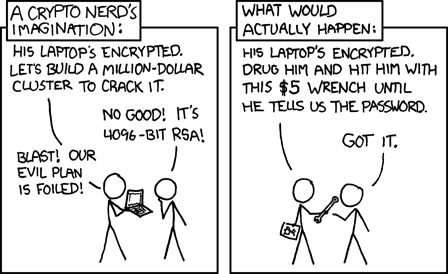
\includegraphics[width=10cm]{security.png}
        \else
            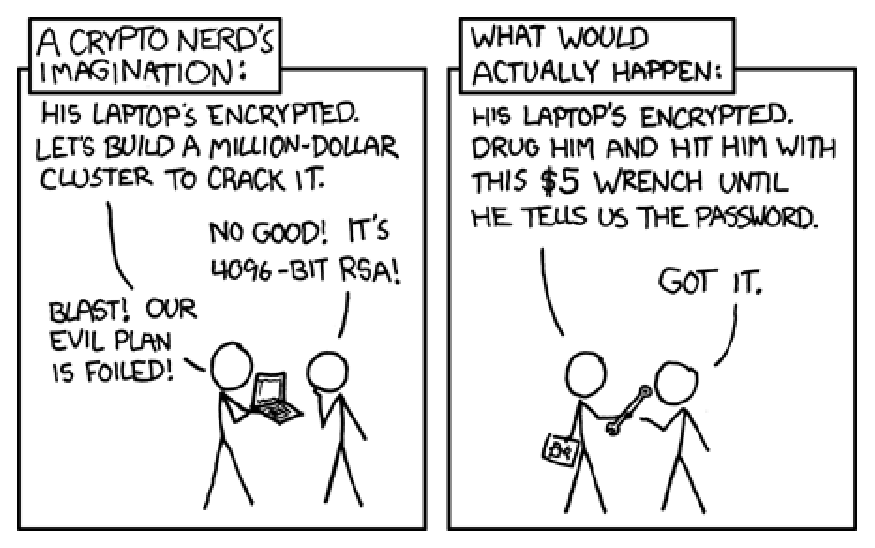
\includegraphics[width=10cm]{security.eps}
        \fi

        \url{http://xkcd.com/538/}. Ce dessin est publié sous licence \href{http://creativecommons.org/licenses/by-nc/2.5/}{ Creative Commons Attribution-NonCommercial 2.5 License}.
\end{center}

\noindent \ldots tout dépends du contexte.

%---------------------------------------------------------------------------------------------------------------------------
\subsection{Anneaux principaux et polynômes}
%---------------------------------------------------------------------------------------------------------------------------

Nous supposons que \( \eK\) est une corps commutatif, et nous étudions l'anneau \( \eK[X]\). Étant donné que \( \eK\) est commutatif pour tout polynôme que l'idéal engendré par \( P\) est \( (P)=\eK[X]P\), voir la notation \eqref{EqDefxMkDtW}.

\begin{remark}
    Un polynôme est irréductible dans \( \eK[X]\) au sens de la définition \ref{DeirredBDhQfA} si et seulement si il est irréductible au sens de la définition \ref{DefIrredfIqydS} parce que seules les constantes (non nulles) sont inversibles dans \( \eK[X]\).
\end{remark}

\begin{corollary}       \label{CorsLGiEN}
    Si \( \eK\) est un corps et si \( P\) est un polynôme irréductible de degré \( n\), alors l'ensemble \( \eL=\eK[X]/(P)\) est un corps. De plus \( \eL\) est un espace vectoriel de dimension \( n\).
\end{corollary}

\begin{proof}
    En effet \( \eK[X]\) est un anneau principal par le théorème \ref{ThoCCHkoU}, par conséquent la proposition \ref{PropoTMMXCx} déduit que \( \eK[X]/(P)\) est un corps.

    Une base de \( \eL\) est donnée par les projections de \( 1,X,X^2,\ldots, X^n\).
\end{proof}

%+++++++++++++++++++++++++++++++++++++++++++++++++++++++++++++++++++++++++++++++++++++++++++++++++++++++++++++++++++++++++++
\section{Corps de rupture, corps de décomposition}
%+++++++++++++++++++++++++++++++++++++++++++++++++++++++++++++++++++++++++++++++++++++++++++++++++++++++++++++++++++++++++++

\begin{lemma}       \label{LemobATFP}
    Soit \( \eL\) un corps fini et \( \eK\) un sous corps de \( \eK\). Alors il existe \( s\in \eN\) tel que
    \begin{equation}        \label{EqUgqlJQ}
        \Card(\eK)=\Card(\eL)^n.
    \end{equation}
\end{lemma}

\begin{proof}
    Le corps \( \eL\) est un \( \eK\)-espace vectoriel de dimension finie. Si \( s\) est la dimension alors nous avons la formule \eqref{EqUgqlJQ} parce que chaque élément de \( \eL\) est un \( s\)-uple d'éléments de \( \eK\).
\end{proof}

\begin{definition}
    Soit \( \eK\) un corps commutatif. Une \defe{extension}{extension!de corps} de \( \eK\) est un corps \( \eL\) muni d'un morphisme \( i\colon \eL\to \eK\). Nous identifions le plus souvent \( \eK\) avec \( i(\eK)\subset \eL\).

    Une extension est \defe{algébrique}{extension!algébrique}\index{algébrique!extension} de \( \eK\) est une extension dont tous les éléments sont racines de polynômes dans \( \eK[X]\).
\end{definition}
Notons que \( \eR\) n'est pas une extension algébrique de \( \eQ\). En effet il existe seulement une infinité \emph{dénombrable} de polynômes dans \( \eQ[X]\) et donc une infinité dénombrable de racines de tels polynômes. Toute extension algébrique de \( \eQ\) est donc dénombrable.

%---------------------------------------------------------------------------------------------------------------------------
\subsection{Polynôme minimal}
%---------------------------------------------------------------------------------------------------------------------------

Soit \( \eL\) une extension de \( \eK\) et \( a\in \eL\). Nous considérons l'idéal
\begin{equation}
    I_a=\{ P\in \eK[X]\tq P(a)=0 \}.
\end{equation}
Étant donné que \( \eK[X]\) est principal, cet idéal est principal et donc accepte un générateur unitaire. Nous nommons ce dernier \defe{polynôme minimal}{polynôme!minimal!d'un élément d'une extension} de \( a\) sur \( \eK\).

\begin{example}
Le polynôme minimal dépends du corps sur lequel on le considère. Par exemple le nombre imaginaire pur \( i\) accepte \( X-i\) comme polynôme minimal sur \( \eC\) et \( X^2+1\) sur \( \eQ[X]\).
\end{example}

Deux éléments \( \alpha\) et \( \beta\) dans \( \eL\) sont dit \defe{conjugués}{conjugués!éléments d'une extension} si ils ont même polynôme minimal. Par exemple \( i\) et \( -i\) sont conjugués dans \( \eC\) vu comme extension de \( \eQ\).

\begin{lemma}[\cite{UQerHHk}]
    Un nombre complexe algébrique dont tous les conjugués sont de module \( 1\) est une racine de l'unité.
\end{lemma}

\begin{lemma}
    Si \( \eL\) est une extension de \( \eK\), alors \( \eL\) est un espace vectoriel sur \( \eK\).
\end{lemma}

\begin{proof}
    Notons que \( \eL\) est un espace vectoriel sur \( \eK\) parce que si \( \lambda\in \eK\) et \( x\in \eL\) nous pouvons considérer la multiplication scalaire
    \begin{equation}
        \lambda\cdot x=i(\lambda)x
    \end{equation}
    où la multiplication du membre de droite est celle du corps \( \eL\). 
\end{proof}

\begin{definition}      \label{DefUYiyieu}
    Le \defe{degré}{degré!extension de corps} de \( \eL\) est la dimension de cet espace vectoriel. Il est noté \( [\eL:\eK]\)\nomenclature[A]{\( [\eL:\eK]\)}{degré d'une extension de corps}; notons qu'il peut être infini.
\end{definition}

\begin{example}
    L'ensemble \( \eC\) est une extension de \( \eR\) et son degré est \( [\eC:\eR]=2\).
\end{example}

\begin{proposition}[\cite{ROZaSWZ}]     \label{PropGWazMpY}
    Si \( \eL\) est une extension du corps \( \eK\) et si \( \eM\) est une extension de \( \eL\), alors les degrés se multiplient :
    \begin{equation}
        [\eM:\eL][\eL:\eK]=[\eM;\eK].
    \end{equation}
\end{proposition}

\begin{proof}
    Soit \( \{ l_i \}\) une base de \( \eL\) sur \( \eK\) et \( \{ m_j \}\) une base de \( \eM\) sur \( \eL\). Un élément de \( \eM\) se note
    \begin{equation}
        \sum_{j}b_jm_j
    \end{equation}
    pour des \( b_j\in \eL\). Chacun de ces \( b_j\) s'écrit comme une combinaison des \( l_i\) :
    \begin{equation}
        \sum_{j}b_jm_j=\sum_{ij}(a_{ji}l_i)m_j,
    \end{equation}
    donc nous voyons que les éléments \( l_im_j\) de \( \eM\) sont une base de \( \eM\) sur \( \eK\).
\end{proof}

\begin{definition}  \label{DefZCYIbve}
    Soit \( \eL\) une extension de \( \eK\) et \( A\subset \eL\). 
    \begin{enumerate}
        \item
            
    Nous notons \( \eK(A)\)\nomenclature[A]{$\eK(A)$}{corps contenant \( \eK\) et \( A\)} le plus petit sous corps de \( \eL\) qui contient \( \eK\) et \( A\). 
\item
    Nous notons \( \eK[A]\)\nomenclature[A]{$\eK[A]$}{anneau contenant \( \eK\) et \( A\)} le plus petit sous anneau de \( \eL\) qui contienne \( \eK\) et \( A\).
    \end{enumerate}
    Nous disons que l'extension \( \eL\) de \( \eK\) est \defe{monogène}{monogène!extension de corps} ou \defe{\wikipedia{fr}{Extension_simple}{simple}}{extension!simple}\index{simple!extension de corps} si il existe \( \theta\in\eL\) tel que \( \eL=\eK(\theta)\). Un tel élément \( \theta\) est dit \defe{élément primitif}{primitif!élément d'une extension de corps}\index{élément!primitif} de \( \eL\). Il n'est pas nécessairement unique.
\end{definition}

\begin{example}
    Nous avons déjà vu à l'occasion de la définition \ref{DefRGOooGIVzkx} que \( A[X]\) est l'anneau de tous les polynômes de degré fini en \( X\). Cela rentre dans le cadre de la définition \ref{DefZCYIbve} parce un anneau contenant \( X\) doit contenir tous les \( X^n\).

    Notons que même si \( \eK\) est un corps, \( \eK[X]\) reste un anneau parce que \( A/X\) n'est pas dedans. Par contre, \( \eK(X)\) est un corps parce qu'il contient également les fractions rationnelles.
\end{example}

\begin{example} \label{ExLQhLhJ}
    Si nous prenons \( \eF_5\) et que nous l'étendons par \( i\), nous obtenons le corps \( \eK=\eF_5(i)\). Nous savons que tous les éléments \( a\in \eF_5\) sont racines de \( X^5-X\). Mais étant donné que \( i^5=i\), nous avons aussi \( x^5=x\) pour tout \( x\in \eF_5(i)\). Pour le prouver, utiliser le morphisme de Frobenius. Le polynôme \( X^5-X\) est donc le polynôme nul dans \( \eK\).

    Ceci est un cas très particulier parce que nous avons étendus \( \eF_p\) par un élément \( \alpha\) tel que \( \alpha^p=\alpha\). En général sur \( \eF_p(\alpha)\), le polynôme \( X^p-X\) n'est pas identiquement nul, et possède donc au maximum \( p\) racines. Pour \( x\in \eF_p(\alpha)\), nous avons \( x^p=x\) si et seulement si \( x\in \eF_p\).
\end{example}

\begin{lemma}
    Soit \( P\in\eK[X]\) un polynôme unitaire irréductible de degré \( n\). Il existe une extension \( \eL\) de \( \eK\) et \( a\in \eL\) telle que \( \eL=\eK(a)\) et \( P\) est le polynôme minimal de \( a\) dans \( \eL\).
\end{lemma}

\begin{proof}
    Nous prenons \( \eL=\eK[X]/(P)\) où \( (P)\) est l'idéal dans \( \eK[X]\) généré par \( P\). Cela est un corps par le corollaire \ref{CorsLGiEN}. Nous identifions \( \eK\) avec \( \phi(\eK)\) où
    \begin{equation}
        \phi\colon \eK[X]\to \eL 
    \end{equation}
    est la projection canonique. Nous considérons également \( a=\phi(X)\).

    Nous avons alors \( P(a)=0\) dans \( \eL\). En effet \( P(a)=P\big( \phi(X) \big)\) est à voir comme l'application du polynôme \( P\) au polynôme \( X\), le résultat étant encore un élément de \( \eL\). En l'occurrence le résultat est \( P\) qui vaut \( 0\) dans \( \eL\).

    Le polynôme \( P\) étant unitaire et irréductible, il est minimum dans \( \eL\).

    Nous devons encore montrer que \( \eL=\eK(a)\). Le fait que \( \eK(a)\subset \eL\) est une tautologie parce qu'on calcule \( \eK(a)\) dans \( \eL\). Pour l'inclusion inverse soit \( Q(X)=\sum_iQ_iX^i\) dans \( \eK[X]\). Dans \( \eL\) nous avons évidemment \( Q=\sum_iQ_ia^i\).
\end{proof}

\begin{proposition} \label{PropyMTEbH}
    Soit \( \eK\), un corps et \( P\in \eK[X]\) un polynôme. Soient \( a\) et \( b\), deux racines de \( P\) dans (éventuellement) une extension \( \eL\) de \( \eK\). Si \( \mu_a\) et \( \mu_b\) sont les polynômes minimaux de \( a\) et \( b\) (dans \( \eK[X]\)) et si \( \mu_a\neq \mu_b\), alors \( \mu_a\mu_b\) divise \( P\) dans \( \eK[X]\).
\end{proposition}

\begin{proof}
    Nous considérons les idéaux
    \begin{subequations}
        \begin{align}
            I_a=\{ Q\in \eK[X]\tq Q(a)=0 \};
            I_b=\{ Q\in \eK[X]\tq Q(b)=0 \};
        \end{align}
    \end{subequations}
    même si \( Q(a)\) est calculé dans \( \eL\), ce sont des idéaux de \( \eK[X]\). Le polynôme \( \mu_a\) est par définition le générateur unitaire de \( I_a\), et vu que \( a\) est une racine de \( P\), nous avons \( P\in I_a\) et il existe un polynôme \( Q\in \eK[X]\) tel que 
    \begin{equation}    \label{EqvTPoSq}
        P=\mu_aQ.
    \end{equation}

    Montrons que \( \mu_a(b)\neq 0\). En effet supposons que \( \mu_a(b)=0\). Nous avons alors \( \mu_a\in I_b\) et il existe \( R\in \eK[X]\) tel que \( \mu_a=\mu_bR\). Étant donné que \( \mu_b\) divise \( \mu_a\) et que \( \mu_b\neq \mu_a\), nous ne pouvons pas avoir \( \mu_b(a)=0\) parce que \( \mu_b\) divise \( \mu_a\) et que \( \mu_a\) est minimal. Du coup nous devons avoir \( R(a)=0\), ce qui contredirait la minimalité de \( \mu_a\).

    Étant donné que \( \mu_a(b)\neq 0\), l'évaluation de \eqref{EqvTPoSq} en \( b\) montre que \( Q(b)=0\), de telle sorte que \( Q\in I_b\) et il existe une polynôme \( S\) tel que \( Q=\mu_bS\), c'est à dire tel que \( P=\mu_a\mu_bS\), ce qui signifie que \( \mu_a\mu_b\) divise \( P\).
\end{proof}

\begin{example}
    Soit \( P=(X^2+1)(X^2+2)\) dans \( \eR[X]\). Dans \( \eC\) nous avons les racines \( a=i\) et \( b=\sqrt{2}i\) dont les polynômes minimaux sont \( \mu_a=X^2+1\) et \( \mu_2=X^2+2\). Nous avons effectivement \( \mu_a\mu_b\) divise \( P\) dans \( \eR[X]\).

    Si par contre nous considérions les racines \( a=i\) et \( b=-i\), nous aurions \( \mu_a=\mu_n=X^2+1\), et les polynôme \( \mu_a^2\) ne divise pas \( P\).
\end{example}

\begin{proposition}     \label{PropdsRAsk}
    Si \( \eL\) est une extension de \( \eK\) et si \( \alpha\in \eL\) est un élément algébrique sur \( \eK\), alors une base de \( \eL\) comme espace vectoriel sur \( \eK\) est donnée par
    \begin{equation}
        \{ 1,\alpha,\alpha^2,\ldots, \alpha^{n-1} \}
    \end{equation}
    où \( n\) est le degré du polynôme minimal de \( \alpha\) sur \( \eK\).
\end{proposition}

%---------------------------------------------------------------------------------------------------------------------------
\subsection{Corps de rupture}
%---------------------------------------------------------------------------------------------------------------------------

\begin{definition}
    Soit \( P\in\eK[X]\) un polynôme irréductible. Une extension \( \eL\) de \( \eK\) est un \defe{corps de rupture}{corps!de rupture}\index{rupture!corps} pour \( P\) si il existe \( a\in \eL\) tel que \( P(a)=0\) et \( \eL=\eK(a)\).
\end{definition}

\begin{example}     \label{ExemGVxJUC}
    Soit \( \eK=\eQ\) et \( P(X)=X^2-2\). On pose \( a=\sqrt{2}\) et \( \eL=\eQ(\sqrt{2})\subset\eR\). De cette façon \( P\) est scindé :
    \begin{equation}
        P=(X-\sqrt{2})(X+\sqrt{2}).
    \end{equation}
    Le corps \( \eQ(\sqrt{2})\) est donc un corps de rupture pour \( P\).
\end{example}

\begin{example}
    Dans l'exemple \ref{ExemGVxJUC}, le polynôme \( P\) était scindé dans son corps de rupture. Il n'en est pas toujours ainsi. Prenons 
    \begin{equation}
        P(X)=X^3-2
    \end{equation}
    et \( a=\sqrt[3]{2}\). Nous avons, certes, \( P(a)=0\) dans \( \eQ(\sqrt[3]{2})\), mais \( P\) n'est pas scindé parce qu'il y a deux racines complexes.
\end{example}

\begin{example}
    Nous considérons le corps \( \eZ/p\eZ\) où \( p\) est un nombre premier. Si \( s\in \eZ/p\eZ\) n'est pas un carré, alors le polynôme \(P= X^2+s\) est irréductible et un corps de rupture de \( P\) sur \( \eZ/p\eZ\) est donné par \( (\eZ/p\eZ)[X]/(X^2+s)\), c'est à dire l'ensemble des polynômes de degrés \( 1\) en \( \sqrt{s}\). Le cardinal en est \( p^2\).
\end{example}

%---------------------------------------------------------------------------------------------------------------------------
\subsection{Corps de décomposition}
%---------------------------------------------------------------------------------------------------------------------------

\begin{definition}
    Soit \( \eK\) un corps commutatif et \( F=(P_i)_{i\in I}\) une famille d'éléments non constants de \( \eK[X]\). Un \defe{corps de décomposition}{corps!de décomposition}\index{décomposition!corps} de \( F\) est une extension \( \eL\) de \( \eK\) telle que
    \begin{enumerate}
        \item
            les \( P_i\) sont scindés sur \( \eL\),
        \item
            \( \eL=\eK(R)\) où \( R=\bigcup_{i\in I}\{ x\in\eL\tq P_i(x)=0 \}\).
    \end{enumerate}
    C'est à dire que \( \eL\) étends \( \eK\) par toutes les racines de tous les polynômes de \( F\).
\end{definition}

L'unicité est due à la proposition suivante.
\begin{proposition}     \label{PropTMkfyM}
    Soit \( \eK\) un corps et \( P\in\eK[X]\). Soient \( \eL\) et \( \eF\) deux corps de décomposition de \( P\). Alors il existe un isomorphisme \( f\colon \eL\to \eF\) tel que \( f|_{\eK}=\id\).
\end{proposition}
Nous pouvons donc parler du corps de décomposition d'un polynôme.

Soit \( \eK\), un corps et \( \eL\), une extension de \( \eK\). Un élément \( a\in \eL\) est \defe{algébrique}{algébrique!nombre} sur \( \eK\) si il existe un polynôme \( P\in \eK[X]\) tel que \( P(a)=0\).

Une \defe{clôture algébrique}{clôture algébrique} du corps \( \eK\) est une extension algébriquement close de \( \eK\) dont tous les éléments sont algébriques sur \( \eK\).

\begin{remark}
    L'ensemble \( \eC\) n'est pas une clôture algébrique de \( \eQ\) parce qu'il existe des éléments de \( \eC\) qui ne sont pas des racines de polynômes à coefficients rationnels.
\end{remark}
L'existence d'une clôture algébrique pour tout corps est le théorème de Steinitz.
%TODO : à faire, le théorème de Steinitz.

\begin{example}     \label{ExfUqQXQ}
    Soit \( p\) un nombre premier. Montrons que le polynôme 
    \begin{equation}
        Q(X)=X^p-X+1
    \end{equation}
    est irréductible dans \( \eF_p\). 

    Nous supposons qu'il n'est pas irréductible, c'est à dire que
    \begin{equation}
        Q(X)=R(X)S(X)
    \end{equation}
    avec \( R\) et \( S\), des polynômes de degrés \( \geq 1\) dans \( \eF_p[X]\)

    Soit \( \bar\eF_p\) une clôture algébrique de \( \eF_p\) et \( \alpha\in \bar \eF_p\) tel que \( R(\alpha)=0\). Pour tout \( a\in \eF_p\), nous avons
    \begin{subequations}
        \begin{align}
            Q(\alpha+a)&=(\alpha+a)^p-(\alpha+a)+1\\
            &=\alpha^p+a^p-\alpha-a+1\\
            &=\alpha^p-\alpha+1\\
            &=Q(\alpha)\\
            &=0
        \end{align}
    \end{subequations}
    où nous avons utilisé le fait que \( a^p=a\) et que \( \alpha\) était une racine de \( Q\). Ce que nous venons de prouver est que l'ensemble des racines de \( Q\) dans \( \bar\eF_p\) est donné par \( \{ \alpha+a\tq a\in \eF_p \}\).

    Les polynômes \( R\) et \( S\) sont donc formés de produits de termes \( X-(\alpha+a)\) avec \( a\in \eF_p\). L'un des deux --disons \( R\) pour fixer les idées-- doit bien en avoir plus que \( 1\). Nous avons alors
    \begin{equation}
        R(X)=\prod_{i=1}^{k}\big( X-(\alpha+a_i) \big)
    \end{equation}
    où les \( a_i\) sont les éléments de \( \eF_p\). En développant un peu,
    \begin{equation}
        R(X)=X^k-\sum_{i=1}^k(\alpha+a_i^{k-1})+\text{termes de degré plus bas en \( X\)}.
    \end{equation}
    Le coefficient devant \( X^{k-1}\) n'est autre que \( k\alpha+\sum_ia_i\). Étant donné que \( k\neq 0\) et que \( R\in \eF_p[X]\), nous devons avoir \( \alpha\in \eF_p\). Par conséquent nous avons \( \alpha^p=\alpha\) et une contradiction :
    \begin{equation}
        Q(\alpha)=\alpha^p-\alpha+1=1\neq 0.
    \end{equation}

    Le polynôme \( X^p-X+1\) est donc irréductible sur \( \eF_p\).
\end{example}
